\section{拟采用的研究方法、技术路线、实验方案及其可行性分析}

\subsection{基于智能体的漏洞挖掘方法}
\label{sec:discovery-method}

\subsubsection{问题定义与总体技术框架}
\label{sec:discovery-framework}

本研究面向嵌入式设备与剥离符号二进制，重点挖掘协议状态违例、跨调用行为逻辑错误和资源泄漏等不易通过崩溃信号识别的问题。针对行为约束不完整、内部状态难以观察以及错误判据不足等挑战，本文拟提出行为约束引导的状态探索与主动观测方法，将“如何触发潜在错误”与“如何观察并判断错误”联合考虑，通过针对性交互获得可复现的行为违例。

方法以目标设备或可执行二进制，以及能够获得的协议文档、接口说明、配置和正常交互样例为输入，不要求预先提供漏洞位置、触发程序或官方补丁。对于二进制可分析且具备运行时观察条件的目标，结合静态分析与动态观察辨识安全相关状态；对于仅能进行设备交互的目标，则利用响应、后续操作结果及可用诊断信息推断状态，不假设能够获取内部变量或代码覆盖。按照“行为约束构建—状态辨识与主动观测—交互生成与反馈优化—候选漏洞确认”的路线开展，技术路线如图~\ref{fig:mining-route}~所示，输出包含约束依据、触发条件、交互序列及安全影响的漏洞报告。

\begin{figure}[htbp]
\centering
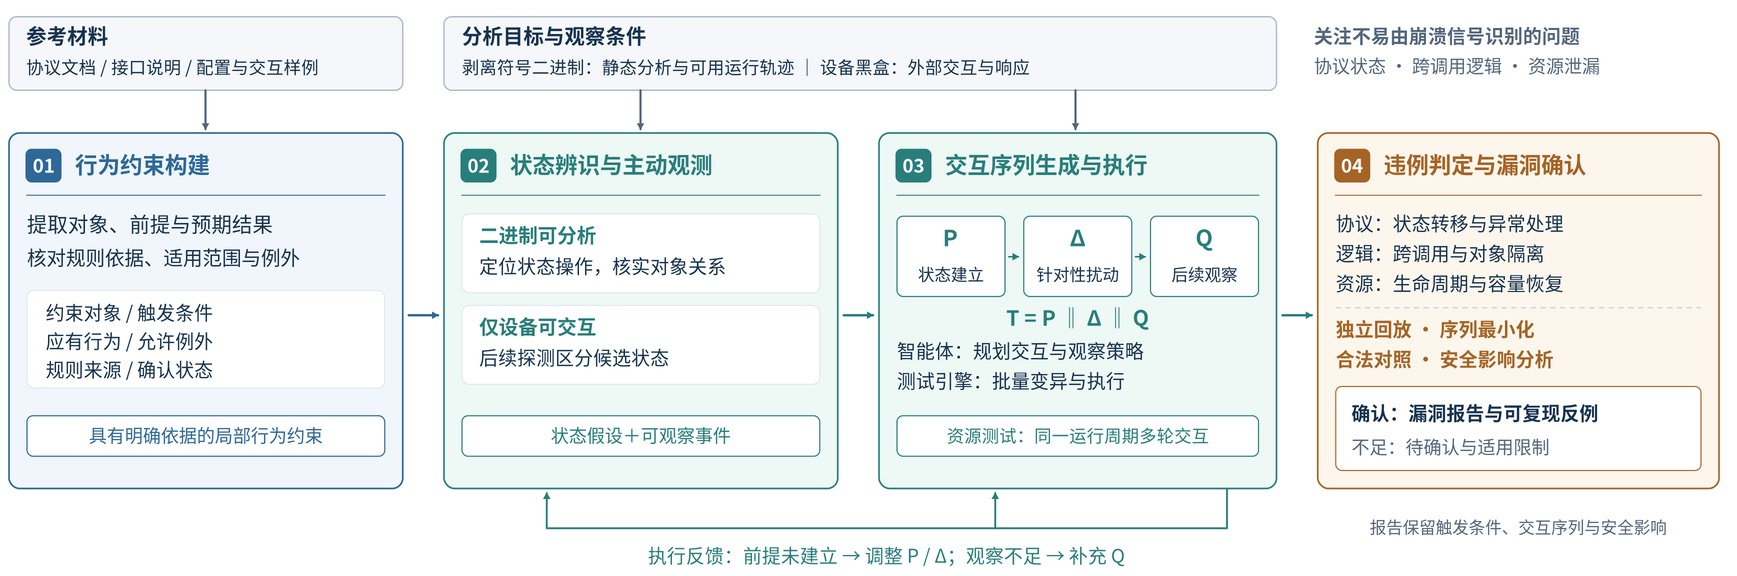
\includegraphics[width=\textwidth]{Img/漏洞挖掘.jpg}
\caption{基于智能体的漏洞挖掘技术路线}
\label{fig:mining-route}
\end{figure}

\subsubsection{行为约束引导的状态探索与主动观测}
\label{sec:discovery-technical-route}

首先，构建具有明确依据和适用范围的局部行为约束。利用大模型分析协议规范、接口说明及历史缺陷模式，提取约束对象、适用前提、触发事件和预期结果，再结合目标实现与交互信息检查其适用条件及事件映射。例如，资源约束不仅描述申请与释放操作，还需明确资源所属的会话、生命周期结束条件，以及允许延迟回收的例外。规则构建区分规范要求与实现观察，不将目标当前表现直接视为正确行为；缺少充分依据的规则保留为待验证假设。

其次，建立行为约束与目标可观察状态之间的对应关系。对于二进制目标，围绕约束涉及的操作定位状态建立、更新、使用和清理位置，并在具备条件时利用运行轨迹核实对象关系。对于黑盒设备，当即时响应不足以辨识状态时，由智能体构造具有区分能力的后续交互。例如，在规范要求注销后权限失效的场景中，除检查注销响应外，还需通过后续受保护操作观察原会话权限是否残留。系统根据结果更新候选状态假设；对可能改变被测状态的探测，通过相同前缀的独立回放进行对照，减少观察操作本身的干扰。

在此基础上，联合构造状态建立、条件扰动与后续观察序列，将一次测试表示为
\begin{equation}
    T = P \Vert \Delta \Vert Q,
    \label{eq:discovery-test-sequence}
\end{equation}
其中，$P$ 为建立目标状态的交互前缀，$\Delta$ 为针对特定约束的扰动，$Q$ 为用于辨识结果的观察后缀，$\Vert$ 表示序列连接。测试在保持无关语法和依赖条件的同时，改变消息顺序、取消时机或断连行为等目标条件，避免因前置步骤无效而始终停留在外围检查。对于资源累积问题，在同一运行周期中重复相关交互，再检查清理后的资源占用与后续申请能力。所有触发均限定在预设的交互能力和有效环境条件内，不以任意修改内部状态代替真实可达过程。

执行过程中，智能体负责约束解释、交互规划和观察策略调整，测试引擎负责批量变异、执行与结果采集。反馈除可获得的代码覆盖外，还包括约束前提是否成立、目标事件是否发生、状态假设是否得到区分以及资源回收条件是否满足。当前提未建立时补充交互前缀，扰动未触及目标行为时调整测试条件，结果无法判定时增加观察后缀，从而将测试预算用于具体的触发或观察缺口。

最后，根据约束类型构造相应判据：协议类检查状态转移及异常消息处理是否符合要求，跨调用逻辑类检查取消、回滚和对象隔离等行为关系，资源类检查生命周期结束后的资源残留与容量恢复。判定针对目标的实际行为，而不是将测试输入不合法直接视为漏洞。资源增长或等待超时仅作为候选信号，需要结合明确的回收条件与正常路径对照排除合法缓存和延迟清理。对候选问题进行独立回放、序列最小化和安全影响分析，排查规约误解与环境偏差；观察不足时保留不确定结论，不以模型判断替代可验证证据。

\subsubsection{实验方案与可行性分析}
\label{sec:discovery-evaluation}

实验拟按照可控软件对象、剥离符号二进制和真实设备逐步开展。在可控对象上利用源码和完整执行信息建立评价依据，但按实验设置限制被测系统能够访问的信息；随后分别评价剥离二进制与设备黑盒条件下的发现能力。测试对象覆盖协议状态、跨调用行为及资源生命周期相关缺陷，已知漏洞回溯与未知漏洞发现分别报告，目标漏洞的官方补丁和事后测试不进入发现阶段。

对比方法包括适用的状态感知模糊测试、规则驱动测试，以及使用相同模型、工具权限和预算的通用智能体。通过移除行为约束、主动观测和反馈调度等模块，评价各项设计的贡献，并比较持续多轮测试与逐轮重置对资源问题发现的影响。主要指标包括独立确认的缺陷与安全漏洞数量、首次确认时间、误报比例、无法判定比例及完整分析成本；状态覆盖与有效交互比例用于解释方法效果，不替代最终漏洞判定。

实现上拟复用二进制分析、模糊测试和设备交互工具，将新增研究集中于行为约束映射、触发与观察序列的联合生成，以及分类判据的可靠执行。初期选择具备明确协议或接口说明、可重复运行的目标验证核心机制，再逐步扩展至信息和观察能力受限的设备。对于环境难以复现或约束无法确认的案例，记录相应限制并分开分析，以控制实施风险并明确方法适用范围。

\subsection{基于智能体的漏洞自动修复方法}
\label{sec:repair-method}

\subsubsection{问题定义与总体技术框架}
\label{sec:repair-framework}

本研究面向已报告漏洞的源码自动修复，重点解决漏洞表现位置与实际修复位置不一致、上下文信息不完整，以及模型根因推理过早收敛和补丁生成同质化等问题。本文拟采用分层上下文构建、检索增强的多假设根因分析与多策略补丁生成相结合的方法，逐步完成从漏洞相关位置到根因解释、再到候选修复的分析过程，减少对准确修复位置和固定补丁模式的依赖。

方法以项目源码、漏洞相关位置及对应的 漏洞 类别为输入。其中，漏洞相关位置可以是异常触发或表现位置，不要求预先指出应修改的语句或函数。整体按照“漏洞上下文构建—多假设根因分析—多策略补丁生成”的路线开展，通过不同分析角色完成源码裁剪、依赖补全、根因推理和候选生成，无需针对修复任务进行模型微调。系统输出细化后的修复区域、根因分析报告及候选补丁集合，补丁是否满足安全要求则由后续独立验证确认。

\subsubsection{上下文增强与多假设推理驱动的补丁生成}
\label{sec:repair-technical-route}

首先，采用分阶段分析构建漏洞相关上下文。以报告位置为起点，引导大模型沿前向和后向分析数据依赖与控制依赖，保留与漏洞传播、危险操作及其前置条件相关的代码，裁剪无关实现，形成初始切片。随后，由依赖分析角色检查缺失的变量定义、函数调用及隐式状态关联，结合指针别名、共享状态和操作副作用，从源码仓库中补充相关代码。最后，由安全分析角色检查现有上下文是否足以解释漏洞，对缺失的辅助函数、数据结构和领域逻辑继续检索，并重新判断实际需要修改的程序区域。该过程以降低噪声、覆盖根因和保留必要的定义--使用关系为目标，而不是将报告位置直接作为补丁插入位置。

其次，构建支持根因分析的历史漏洞知识库。以 ReposVul 中的真实漏洞修复案例为基础，保存 漏洞 类别、漏洞代码、根因描述和补丁差异，分别对代码与根因文本进行向量化，并按 漏洞 类别组织检索分区。针对当前漏洞，智能体先依据增强后的上下文生成初始根因解释，但仅将其作为检索线索，不直接作为最终结论。随后，在对应类别中分别使用漏洞代码和初始根因描述开展余弦相似度检索，得到代码相似性与根因相似性两个排序列表。

为结合不同检索信号，采用倒数排名融合（Reciprocal Rank Fusion，RRF）计算案例的综合相关性：
\begin{equation}
    \operatorname{RRF}(e)
    =
    \sum_{j \in \{\mathrm{code},\,\mathrm{rca}\}}
    \frac{1}{k + \operatorname{rank}_{j}(e)},
    \label{eq:repair-rrf}
\end{equation}
其中，$e$ 表示历史案例，$\operatorname{rank}_{j}(e)$ 表示其在代码或根因检索通道中的排名，$k$ 为平滑常数。该方法在排序层面融合信息，避免直接拼接较长代码与较短根因描述造成信息不均衡。选取融合排名靠前的案例，将其根因说明和补丁差异作为参考，引导智能体提出多种候选根因解释，再结合初始分析形成结构化根因报告。漏洞 类别用于限定检索范围，而不直接决定当前漏洞的根因或修复模板。

在根因报告形成后，利用更新后的解释再次检索修复案例。具体而言，重新编码最终根因报告，更新根因通道的案例排序，并与已有代码通道排序进行融合，获得更贴近当前漏洞机制的修复参考。与仅在分析开始时检索一次相比，这一步使补丁生成所使用的历史经验能够随根因理解的变化而调整，减少初始解释偏差对后续生成的持续影响。

最后，通过五种互补策略引导补丁生成。最小修复以低侵入性修改直接处理核心根因；稳健修复采用成熟的安全实现替换危险编码模式；架构修复通过设计层面的调整减少产生危险行为的可能；增强型最小修复在局部修改基础上补充稳健性检查；局部架构修复结合安全实现替换与局部设计改进，在修改范围和结构调整之间取得平衡。智能体结合漏洞上下文、根因报告与更新后的参考案例，分别生成不同策略下的候选补丁，使候选差异体现在实际修复方式，而不只是代码表述变化。

各候选补丁保留对应的根因解释和修改依据，形成供后续验证的修复集合。本阶段关注有效修复方案的生成与覆盖，不以模型对补丁的自我评价代替正确性验证，也不预设修改最少或最接近官方补丁的方案必然正确。

\subsubsection{实验方案与可行性分析}
\label{sec:repair-evaluation}

实验拟采用 APPATCH 中的真实漏洞案例评价整体修复能力，并利用 InterPVD 中触发位置与修复位置跨函数分离的案例，评价不准确定位条件下的上下文构建与根因重定位能力。历史知识库与测试集按漏洞实例去重，排除测试漏洞对应的修复案例，避免检索直接暴露目标补丁。系统可访问漏洞源码、报告位置和类别信息，参考补丁仅用于评价，不进入目标漏洞的生成过程。

对比方法包括直接提示生成、APPATCH，以及 VulRepair、VulMaster 等修复方法。其中，提示式方法在相同基础模型和候选生成预算下进行比较，训练式方法则按其模型配置独立报告。主要指标包括修复召回率、补丁准确率和 F1 值：修复召回率衡量至少获得一个正确候选的漏洞比例，补丁准确率衡量生成候选中正确补丁的比例；同时统计根因分析准确率、不同模型下的表现及单例时间和推理成本。

\subsection{基于智能体的漏洞修复验证方法}

\textbf{拟解决的关键问题}：智能体在端到端漏洞修复验证（以补丁存在性测试为核心任务）中的两大瓶颈——\textbf{剥离二进制中的补丁定位}与\textbf{演化补丁识别}。前期实证研究表明，前者占弱模型配置独有失败的 95.2\%，后者是鲁棒性测试的主要失分点~\cite{zhang2026agenticppt}。两者本质上都源于跨抽象层次补丁语义对齐困难、修复意图难以形式化：源码级补丁意图与二进制级指令序列之间存在语义鸿沟，且现有方法过度依赖补丁的形式特征而非修复意图。

\textbf{技术方案}：针对上述问题，本文提出\textbf{语义先验引导的智能体修复验证增强框架}，整体技术路线如图~\ref{fig:verify-route} 所示，包含三个核心模块：

\begin{figure}[htbp]
\centering
\begin{tikzpicture}[node distance=0.45cm]
  \node[module] (m1) {%
    \textbf{模块一：漏洞语义先验提取}（离线，一次/漏洞）\\
    CVE 描述 + 补丁 diff + 源码上下文 $\xrightarrow{\text{智能体推理}}$\\
    漏洞语义五元组 $\langle$触发条件, 危险操作, 干预点, 修复意图, 上下文$\rangle$};
  \node[module, below=of m1] (m2) {%
    \textbf{模块二：语义引导的补丁定位}（在线，核心创新）\\
    粗定位：字符串/常量/导入表启发式 $\rightarrow$ 候选函数集\\
    细定位：五元组约束 + 反汇编切片 $\rightarrow$ Top-K 补丁候选区\\
    置信度排序：基于语义匹配度的候选排序};
  \node[module, below=of m2] (m3) {%
    \textbf{模块三：演化补丁的语义等价判定}（在线，核心创新）\\
    干预点识别：定位补丁实际修改的二进制指令\\
    修复意图比对：判断干预是否实现"修复意图"（而非形式匹配）\\
    不变式检查：验证修复后是否满足语义不变式};
  \draw[arr] (m1) -- (m2);
  \draw[arr] (m2) -- (m3);
\end{tikzpicture}
\caption{基于智能体的漏洞修复验证技术路线}
\label{fig:verify-route}
\end{figure}

\begin{itemize}
  \item \textbf{模块一：漏洞语义先验提取}。离线阶段利用智能体从 CVE 描述、补丁 diff 与源码上下文中提取漏洞语义五元组，作为统一语义先验，替代现有方法仅依赖原始补丁 diff 的浅层表示。
  \item \textbf{模块二：语义引导的补丁定位}。在线阶段采用"粗—细"两阶段定位：先用传统启发式（字符串、常量、导入表）快速缩小候选函数集，再将五元组作为约束注入智能体推理，引导其在候选函数中进行语义切片与置信度排序，输出 Top-K 补丁候选区域。
  \item \textbf{模块三：演化补丁的语义等价判定}。针对同一漏洞可能存在多种实现形式的修复（重构、拆分、合并等），不再追求"形式上的补丁匹配"，而是让智能体判断目标二进制中的干预点是否\textbf{实现了与原始补丁相同的修复意图}，并通过语义不变式进行交叉验证。
\end{itemize}

\textbf{可行性分析}：（1）数据基础充分：已构建 561 CVE 高保真基准与 12 组智能体配置的运行日志~\cite{zhang2026pptempirical,zhang2026agenticppt}，包含大量补丁定位与演化补丁的成功/失败案例，可直接用于方法设计与消融验证；（2）技术路线有实证支撑：前期工作已证明"丰富补丁元数据提升 DSR"与"补丁定位是主要瓶颈"两个关键结论，本方案是这两个结论的直接延伸，技术风险低；（3）工具链成熟：智能体框架（Codex / MiniSWEAgent）、二进制分析工具（binutils / Ghidra）与评估基准均已就绪，可快速进入实验迭代。

\textbf{实验方案}：基准沿用前期 561-CVE Source-Built Benchmark + Patch Evolution Set + Ubuntu Packages Set；对比方法包括 Codex 原始配置、Lares~\cite{lares}、PPTSP~\cite{pptsp}、PS\textsuperscript{3}~\cite{ps3}、BinXray~\cite{binxray}；评估指标包括 DSR、Accuracy、补丁定位准确率、每例 token 成本与时延；消融实验分别验证三个模块的独立贡献。预期全配置 DSR $\geq$ 0.98，演化补丁子集 DSR 提升 $\geq$ 15\%，成本增加 $\leq$ 10\%；进一步将验证能力对偶迁移至修复场景，在 RRBench 生成补丁上验证修复正确性判定的有效性。